\subsection{Growth Versus Business Cycle Effects} \label{subsec:detrend}

Economists separate movements of macroeconomic series into two distinct categories: growth effects and business cycle effects \parencite{stulz1985macroeconomic}. Growth effects, typically measured using decade-to-decade long-run economic trends, are determined by a country's pace of idea generation, strength of institutions, and other more stagnant factors \parencites{acemoglu2001colonial}{jones2016facts}{jones2019paul}. Business cycles, in contrast, include short-run economic fluctuations caused by policy decisions, international events, and other unpredictable shocks \parencites{lucas1995understanding}{mitchell2024business}. This paper exclusively focuses on understanding the business cycle consequences of fiscal policy.

Figure \ref{fig:growth-effects} shows US real GDP per capita from 1952 to 2007. Over time, long-run growth is very consistent and follows a linear-in-logs trend. This long-run constant growth is well-documented across the world in growth rates for key macroeconomic series \parencites{papell2014long}.\footnote{There have been a handful of instances where this breaks, including the so-called ``growth miracles'' in East Asia \parencite{easterly199511} and the post-Great Recession growth slowdowns \parencites{benigno2018stagnation}. For the purposes of this paper, we treat long-run constant growth as a fact.} This constant trend is also key for isolating business cycle effects; fluctuations around the constant growth path can be viewed as exclusively business cycle effects.

\begin{figure}[t]
    \centering
    \caption{US real GDP per capita over time (1952-2007)}
    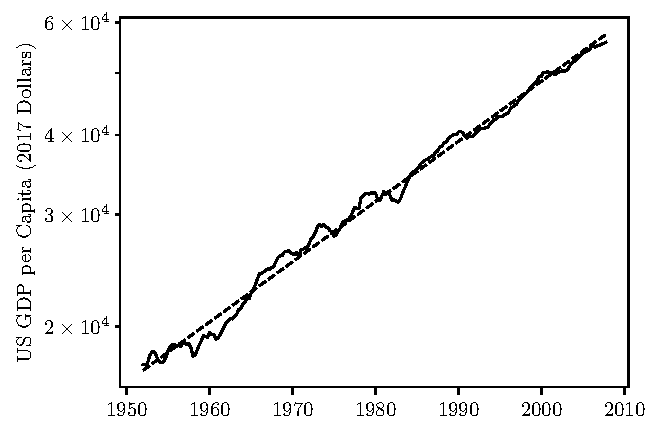
\includegraphics{figures/growth_effects.pdf}

    {\scriptsize \emph{Notes:} Dashed best fit line calculated using OLS.}
    \label{fig:growth-effects}
\end{figure}

Numerically, for an economic series $y_t$ we use the log-deviation from trend $\hat{y}_t$ as its business cycle effect. To calculate this, we run the regression
\[
    \log y_t = \alpha_0 + \alpha_1 t + \hat{y}_t
\]
where $\alpha_0$ and $\alpha_1$ determine the long-run trend for the series and the error term $\hat{y}_t$ is the indicator's business cycle deviations from the trend \parencite{seip2024scoring}.\footnote{For interpretability, we multiply this by 100 in all of our results and figures. Since deviations from trend, at least within the United States, are small, this can be thought of as the ``percent deviation from trend'' of the indicator.} This method can be overly simplistic for data that exhibits significant changes in growth rates over time, but our exclusive focus is on the effect of policy decisions within the United States, a country that has had consistent trends over time, avoiding these concerns.


\subsection{The Reduced-Form VAR}

Our strategy to estimate the causal effect of fiscal policy decisions on GDP uses a VAR. The reduced-form of a VAR assumes a vector of outputs follows an autoregressive process with respect to the whole vector \parencite{neusser2016time}. Like standard univariate autoregressive models, the order of the VAR determines the number of lags included in the model. Unlike univariate autoregressive models, we model a variable using lags for the full set of outputs in the model, not just one.

\begin{figure}[t!]
    \centering
    \caption{Order one, three variable, reduced-form VAR causal graph}
    \begin{psmatrix}[colsep=1.5cm, rowsep=1cm]
    % nodes
    $\dots$ & $y_{1, t-3}$ & $y_{1, t-2}$ & $y_{1, t-1}$ & $y_{1, t}$ \\
    $\dots$ & $y_{2, t-3}$ & $y_{2, t-2}$ & $y_{2, t-1}$ & $y_{2, t}$ \\
    $\dots$ & $y_{3, t-3}$ & $y_{3, t-2}$ & $y_{3, t-1}$ & $y_{3, t}$

    % first column of arrows
    \ncline[nodesep=5pt]{->}{1,1}{1,2}
    \ncline[nodesep=5pt]{->}{1,1}{2,2}
    \ncline[nodesep=5pt]{->}{1,1}{3,2}
    \ncline[nodesep=5pt]{->}{2,1}{1,2}
    \ncline[nodesep=5pt]{->}{2,1}{2,2}
    \ncline[nodesep=5pt]{->}{2,1}{3,2}
    \ncline[nodesep=5pt]{->}{3,1}{1,2}
    \ncline[nodesep=5pt]{->}{3,1}{2,2}
    \ncline[nodesep=5pt]{->}{3,1}{3,2}

    % second column
    \ncline[nodesep=5pt]{->}{1,2}{1,3}
    \ncline[nodesep=5pt]{->}{1,2}{2,3}
    \ncline[nodesep=5pt]{->}{1,2}{3,3}
    \ncline[nodesep=5pt]{->}{2,2}{1,3}
    \ncline[nodesep=5pt]{->}{2,2}{2,3}
    \ncline[nodesep=5pt]{->}{2,2}{3,3}
    \ncline[nodesep=5pt]{->}{3,2}{1,3}
    \ncline[nodesep=5pt]{->}{3,2}{2,3}
    \ncline[nodesep=5pt]{->}{3,2}{3,3}

    % third column
    \ncline[nodesep=5pt]{->}{1,3}{1,4}
    \ncline[nodesep=5pt]{->}{1,3}{2,4}
    \ncline[nodesep=5pt]{->}{1,3}{3,4}
    \ncline[nodesep=5pt]{->}{2,3}{1,4}
    \ncline[nodesep=5pt]{->}{2,3}{2,4}
    \ncline[nodesep=5pt]{->}{2,3}{3,4}
    \ncline[nodesep=5pt]{->}{3,3}{1,4}
    \ncline[nodesep=5pt]{->}{3,3}{2,4}
    \ncline[nodesep=5pt]{->}{3,3}{3,4}

    % second column
    \ncline[nodesep=5pt]{->}{1,4}{1,5}
    \ncline[nodesep=5pt]{->}{1,4}{2,5}
    \ncline[nodesep=5pt]{->}{1,4}{3,5}
    \ncline[nodesep=5pt]{->}{2,4}{1,5}
    \ncline[nodesep=5pt]{->}{2,4}{2,5}
    \ncline[nodesep=5pt]{->}{2,4}{3,5}
    \ncline[nodesep=5pt]{->}{3,4}{1,5}
    \ncline[nodesep=5pt]{->}{3,4}{2,5}
    \ncline[nodesep=5pt]{->}{3,4}{3,5}
\end{psmatrix}

    \label{fig:rfvar-graph}
\end{figure}

Figure \ref{fig:rfvar-graph} demonstrates the assumed causal graph for a three variable, order one VAR. At each time $t$, the whole vector of outputs $Y_t = (y_{1, t}, y_{2, t}, y_{3, t})'$ depends on the whole vector at time $t-1$. Causal pathways lead from $y_{1, t-1}$, $y_{2, t-1}$, and $y_{3, t-1}$ into $y_{1,t}$. A higher order VAR extends this so $Y_t$ depends on more past versions of itself. For example, a second order model would assume $Y_t$ depends on $Y_{t-1}$ and $Y_{t-2}$.

The estimating equation for an order $p$ VAR with $n$ outputs is given by
\[
    Y_t = \sum_{\ell = 1}^p B_\ell Y_{t - \ell} + u_t
\]
where $Y_t$ is the $n \times 1$ vector of outputs we are interested in modeling, $B_{\ell}$ is the $n \times n$ coefficient matrix, and $u_t$ is the $n \times 1$ vector of multivariate-normal error terms with variance-covariance matrix $\Sigma$. The terms in $u_t$ represent unexpected movements of the series in the model potentially caused by international events and movements in excluded macroeconomic series.


\subsection{Correlated and Structural Shocks}

Reduced form VARs are effective tools for understanding associations between variables and for forecasting, but fail to differentiate between causation and correlation \parencite{stock2001vector}. This is because the covariance terms in the variance-covariance matrix $\Sigma$ are symmetric, meaning the association between two series goes both ways. Therefore, the error term includes both contemporaneous responses to other series in the model and structural shocks, or causal exogenous movements of a single series in the model. Therefore, reduced form VARs only have a causal interpretation when variables are assumed to have no contemporaneous causal relationships.

Fluctuations in macroeconomic series are assumed to be very interrelated \parencites{sims1980macroeconomics}{shapiro1988sources}{blanchard1988dynamic}{cochrane1994shocks}{nakamura2018identification}. The Federal Reserve sets the interest rate based on the opinions and forecasts of hundreds of economists about the current state of the economy, so understanding how the interest rate affects the economy requires separating the contemporaneous effect of the state of the economy on the interest rate from the effect of the interest rate on the economy \parencite{nakamura2018identification}. Variation in the interest rate standard statistical methods would identify off of could be caused by changes in the overall economy, obscuring the actual effect.

To determine the causal effect of fiscal policy on output, we need to separate these contemporaneous relationships from actual structural shocks. Forward-looking household behavior, tax schemes that take a fraction of incomes, and revenue-based spending decisions by policymakers mean many contemporaneous relationships exist that will confound this relationship \parencites{blanchard2002empirical}{gali2020effects}.


\subsection{Structural VAR} \label{subsec:svar}

To isolate the effects of structural shocks from contemporaneous relationships, we use a structural VAR. A structural VAR adds an additional coefficient matrix to the left-hand side of the estimating equation to get
\[
    A_0 Y_t = \sum_{\ell = 1}^p A_\ell Y_{t - \ell} + \varepsilon_t
\]
where $A_0$ is the matrix of contemporaneous relationships, $A_\ell = A_0 B_\ell$ is the matrix of lagged coefficients, and $\varepsilon_t = A_0 u_t$ is the structural error term \parencite{neusser2016time}. Unlike the reduced-form error term, the variance-covariance matrix of the structural error term is the $n \times n$ identity matrix $I_n$.\footnote{Normalizing the variances to 1 is not strictly necessary; identification only requires the covariances to be zero. The benefit to this normalization is that when we shock the model we measure the effects of a ``typical'' shock.}

To fit the structural VAR, we need to assume which relationships exist within the contemporaneous matrix $A_0$. Specifically, we need to fix $\begin{pmatrix} n \\ 2 \end{pmatrix}$ coefficients within this matrix and then can estimate the remaining coefficients as simultaneous relationships \parencite{neusser2016time}. Importantly, within certain $A_0$ matrix structures, a series can be contemporaneously affected by a structural shock to a series we do not enforce a relationship with through some other intermediate factor. These feedback effects within the matrix are the benefit to SVAR estimation, which calculates $A_0$ using the $\Sigma$ matrix, as opposed to row-wise OLS estimation.

\begin{figure}[t!]
    \centering
    \caption{Order one, three variable, structural VAR causal graph}
    \begin{psmatrix}[colsep=1.5cm, rowsep=1cm]
    % nodes
    $\dots$ & $y_{1, t-3}$ & $y_{1, t-2}$ & $y_{1, t-1}$ & $y_{1, t}$ \\
    $\dots$ & $y_{2, t-3}$ & $y_{2, t-2}$ & $y_{2, t-1}$ & $y_{2, t}$ \\
    $\dots$ & $y_{3, t-3}$ & $y_{3, t-2}$ & $y_{3, t-1}$ & $y_{3, t}$

    % first column of arrows
    \ncline[nodesep=5pt]{->}{1,1}{1,2}
    \ncline[nodesep=5pt]{->}{1,1}{2,2}
    \ncline[nodesep=5pt]{->}{1,1}{3,2}
    \ncline[nodesep=5pt]{->}{2,1}{1,2}
    \ncline[nodesep=5pt]{->}{2,1}{2,2}
    \ncline[nodesep=5pt]{->}{2,1}{3,2}
    \ncline[nodesep=5pt]{->}{3,1}{1,2}
    \ncline[nodesep=5pt]{->}{3,1}{2,2}
    \ncline[nodesep=5pt]{->}{3,1}{3,2}
    \ncline[nodesep=5pt]{->}{1,2}{2,2}
    \ncarc[nodesep=5pt,arcangle=-15]{->}{2,2}{3,2}
    \ncarc[nodesep=5pt,arcangle=-15]{->}{3,2}{2,2}

    % second column
    \ncline[nodesep=5pt]{->}{1,2}{1,3}
    \ncline[nodesep=5pt]{->}{1,2}{2,3}
    \ncline[nodesep=5pt]{->}{1,2}{3,3}
    \ncline[nodesep=5pt]{->}{2,2}{1,3}
    \ncline[nodesep=5pt]{->}{2,2}{2,3}
    \ncline[nodesep=5pt]{->}{2,2}{3,3}
    \ncline[nodesep=5pt]{->}{3,2}{1,3}
    \ncline[nodesep=5pt]{->}{3,2}{2,3}
    \ncline[nodesep=5pt]{->}{3,2}{3,3}
    \ncline[nodesep=5pt]{->}{1,3}{2,3}
    \ncarc[nodesep=5pt,arcangle=-15]{->}{2,3}{3,3}
    \ncarc[nodesep=5pt,arcangle=-15]{->}{3,3}{2,3}

    % third column
    \ncline[nodesep=5pt]{->}{1,3}{1,4}
    \ncline[nodesep=5pt]{->}{1,3}{2,4}
    \ncline[nodesep=5pt]{->}{1,3}{3,4}
    \ncline[nodesep=5pt]{->}{2,3}{1,4}
    \ncline[nodesep=5pt]{->}{2,3}{2,4}
    \ncline[nodesep=5pt]{->}{2,3}{3,4}
    \ncline[nodesep=5pt]{->}{3,3}{1,4}
    \ncline[nodesep=5pt]{->}{3,3}{2,4}
    \ncline[nodesep=5pt]{->}{3,3}{3,4}
    \ncline[nodesep=5pt]{->}{1,4}{2,4}
    \ncarc[nodesep=5pt,arcangle=-15]{->}{2,4}{3,4}
    \ncarc[nodesep=5pt,arcangle=-15]{->}{3,4}{2,4}

    % second column
    \ncline[nodesep=5pt]{->}{1,4}{1,5}
    \ncline[nodesep=5pt]{->}{1,4}{2,5}
    \ncline[nodesep=5pt]{->}{1,4}{3,5}
    \ncline[nodesep=5pt]{->}{2,4}{1,5}
    \ncline[nodesep=5pt]{->}{2,4}{2,5}
    \ncline[nodesep=5pt]{->}{2,4}{3,5}
    \ncline[nodesep=5pt]{->}{3,4}{1,5}
    \ncline[nodesep=5pt]{->}{3,4}{2,5}
    \ncline[nodesep=5pt]{->}{3,4}{3,5}
    \ncline[nodesep=5pt]{->}{1,5}{2,5}
    \ncarc[nodesep=5pt,arcangle=-15]{->}{2,5}{3,5}
    \ncarc[nodesep=5pt,arcangle=-15]{->}{3,5}{2,5}
\end{psmatrix}

    \label{fig:svar-graph}
\end{figure}

Figure \ref{fig:svar-graph} shows an example causal graph for a structural VAR. Since the output vector has three series, we can enforce three simultaneous relationships. In the example, we enforce that $y_1$ causes $y_2$, $y_2$ causes $y_3$, and $y_3$ causes $y_2$. Identification restrictions for the structural VAR can estimate causal effects even along cyclical causal paths. A structural shock to $y_1$ could affect $y_3$ through $y_2$ and a structural shock to $y_2$ would impact $y_2$ through both direct effects from the shock and indirect effects through $y_2$.


\subsection{Estimating Fiscal Multipliers}

To find the effect of a fiscal shock, we estimate the reduced form VAR
\[
    Y_t = \sum_{\ell = 1}^p B_\ell Y_{t - 1} + u_t
\]
where $Y_t = (\hat{x}_t, \hat{g}_t, \hat{t}_t)'$ is a vector of GDP $x_t$, government spending $g_t$, and government revenue $t_t$. Since our data is quarterly, in our preferred specification we use $p = 4$ corresponding to a total period of one year. We choose this since taxes are often paid at an annual frequency, so including one year of lags captures the relevant revenue data over the entire time span \parencite{blanchard2002empirical}. The error term $u_t = (u_t^x, u_t^g, u_t^t)'$ has nonzero covariance, meaning the relationships predicted by the VAR and within the coefficient matrices $B_\ell$ are correlations and not causal.

To identify the causal effect, we implement the model from \textcite{blanchard2002empirical}. We assume
\begin{align*}
    u_t^x &= a_1 u_t^g + a_2 u_t^t + \varepsilon_t^x \\
    u_t^g &= b_1 u_t^x + b_2 \varepsilon_t^t + \varepsilon_t^g \\
    u_t^t &= c_1 u_t^x + c_2 \varepsilon_t^g + \varepsilon_t^t
\end{align*}
where $\varepsilon_t = (\varepsilon_t^x, \varepsilon_t^g, \varepsilon_t^t)'$ is the vector of mutually uncorrelated structural shocks.\footnote{Technically, to fit this system within the framework from Section \ref{subsec:svar} it would need to be rearranged. This formulation is known as the ``AB-model,'' which allows for two structural shocks to show up in the same equation \parencite{lutkepohl2005new}. The interpretations and general concepts of the ``AB-model'' and ``A-model'' introduced earlier are identical, so we ignore this difference.} The first equation enforces that unexpected movements in GDP can be caused by unexpected movements in government spending, government revenue, or structural shocks to GDP. The second enforces that unexpected movements in government spending are caused by unexpected movements in GDP or structural shocks to government revenue or spending. The third equation enforces that unexpected movements in government revenue are caused by unexpected movements in GDP or structural shocks to government spending or revenue.

As is, this system is underidentified, meaning we need to add additional conditions to make the model estimatable. We follow the procedure from \textcite{blanchard2002empirical} that has become standard when estimating the fiscal multiplier \parencites{ramey2011can}{caldara2017analytics}{deleidi2021quantifying}. First, we set $b_1 = 0$. This assumption is justified by the lack of automatic stabilizers for government spending in the US economy \parencites{caldara2017analytics}. Then, we fix $c_1$ using external estimates for the response of government revenue to economic activity. Following \textcite{lutz2010fiscal}, we set $c_1 = 1.7$. Finally, to differentiate between government spending and revenue structural shocks, we set either $b_2$ or $c_2$ to 0. Like \textcite{blanchard2002empirical}, we present two alternative specifications: one where $b_2 = 0$, meaning government spending is decided before revenue, and another where $c_2 = 0$, meaning government revenue is decided before spending. Figure \ref{fig:causal-graph} shows a causal graph for the pathways between the estimated structural shocks and unexpected movements in the outcomes of interest. The causal pathways affecting GDP, government revenue, and government spending therefore include the pathways affecting unexpected movements in Figure \ref{fig:causal-graph} as well as the autoregressive processes.

\begin{figure}[t]
    \centering
    \caption{Causal graph for unexpected movements in GDP, government spending, and revenue}
    \begin{psmatrix}[colsep=3cm, rowsep=1cm]
    % nodes
    $u_t^x$ & $\varepsilon_t^x$ \\
    $u_t^g$ & $\varepsilon_t^g$ \\
    $u_t^t$ & $\varepsilon_t^t$

    % first column of arrows
    \ncline[nodesep=5pt]{->}{2,1}{1,1}
    \ncarc[nodesep=5pt,arcangle=15]{->}{3,1}{1,1}
    \ncarc[nodesep=5pt,arcangle=-25,linewidth=1.5pt]{->}{1,1}{3,1}
    \ncline[nodesep=5pt]{->}{1,2}{1,1}
    \ncline[nodesep=5pt]{->}{2,2}{2,1}
    \ncline[nodesep=5pt]{->}{3,2}{3,1}
    \ncline[nodesep=5pt,linestyle=dashed,dash=3pt 2pt]{->}{2,2}{3,1}
    \ncline[nodesep=5pt,linestyle=dashed,dash=3pt 2pt]{->}{3,2}{2,1}
\end{psmatrix}

    \label{fig:causal-graph}
\end{figure}

This identification strategy relies on many assumptions about the structure of the causal relationships between movements and structural shocks. An alternative strategy from \textcite{mountford2009effects} instead imposes a penalty function on the long-run effects of a structural shock. Estimations using this approach tend to be similar to those using the \textcite{blanchard2002empirical} method we employ. Other strategies that impose conditions on the reduced form of the VAR using sign restrictions or Bayesian techniques but allow for identification of the structural shocks under a weaker set of assumptions are outside the scope of this paper.
